\documentclass[11pt]{article}
\usepackage[margin=1in]{geometry}
\usepackage{amsmath,amssymb}
\usepackage{booktabs}
\usepackage{graphicx}
\usepackage{hyperref}
\usepackage{xcolor}
\graphicspath{{../results/}}

\newcommand{\todo}[1]{\textcolor{red}{\textbf{[TODO: #1]}}}

\title{SurgeryNet: A Graph Neural Decoder for Lattice Surgery}
\author{}
\date{\today}

\begin{document}
\maketitle

\begin{abstract}
Neural decoders for quantum error correction are trained and evaluated almost
entirely on quantum \emph{memory} experiments -- a single static code patch,
held still. Real fault-tolerant computation requires logical gates, which on
surface codes are implemented by lattice surgery: patches merge and split, the
decoding graph changes shape mid-computation, and the effective code distance
varies with time. A neural decoder with a fixed-size input has no valid input
shape during this operation; it cannot be evaluated on lattice surgery at all,
not merely evaluated poorly. A graph neural network has no such constraint.
Among \emph{learned} decoders -- which now outperform minimum-weight perfect
matching (MWPM) on memory experiments -- architecture determines whether the
decoder can operate on lattice surgery at all. We show that fixed-input
architectures cannot transfer, that a graph neural network (GNN) can, and we
report learned-decoder accuracy numbers on merge/split operations, including
timelike (parity-measurement) error rates, together with a real
hyperparameter search that narrows -- but does not close -- the gap to MWPM
on plain memory, and a spacelike/timelike threshold sweep. We report all of
this, including where it did not go as hoped: the GNN still trails MWPM
everywhere in this study, and -- isolated by a controlled comparison, not
merely observed -- training the model longer and on more memory data made
zero-shot transfer to lattice surgery \emph{worse}, not better, regardless
of architecture.
\end{abstract}

\section{Introduction}

Every widely-cited neural decoder result -- AlphaQubit \cite{alphaqubit}, GNN
decoders, transformer decoders -- is a \emph{memory experiment}: prepare a
logical state, run $r$ rounds of stabilizer measurement, check whether it
survived. This is the quantum equivalent of benchmarking a CPU on idle.
Universal fault-tolerant computation requires logical \emph{gates}, and on
surface codes these are implemented by lattice surgery: two patches are
merged by measuring joint stabilizers across a routing region, held merged
for $d$ rounds, then split \cite{horsman2012}.

During that window the decoding problem changes. New detector vertices
appear where patches join. Boundaries move. The effective code distance is
time-varying, and in the worst case the merged patch spans the whole device.
A neural decoder with a fixed-size input cannot be run on it at all -- not
``runs badly,'' but has no valid input shape. A GNN over detection events has
no such constraint. That structural mismatch, not a small accuracy
improvement, is this paper's central claim.

\subsection{The gap}

A 2026 survey of maximum-likelihood decoding states the situation directly:
research to date has focused on memory experiments, whereas universal
fault-tolerant computation requires executing logical gates via lattice
surgery, braiding, or transversal operations, and these operations create
geometrically complex, irregular spacetime decoding graphs that differ
fundamentally from the regular lattice structures of memory experiments
\cite{mld2026}. A real-time decoding review adds a second, independent gap:
high thresholds for space-like \emph{and} time-like errors under lattice
surgery still need to be demonstrated \cite{realtime2023}. Timelike errors
corrupt the parity-measurement outcome rather than the stored state and have
no analogue in a memory experiment; almost nobody reports them. An August
2026 survey of ML approaches to decoding confirms the framing from the
learning side: benchmark review in that literature focuses primarily on
quantum memory experiments \cite{mlsurvey2026}.

Existing systems-level work on lattice surgery decoding -- FPGA/CPU hybrid
spatially-parallel decoding \cite{latte2025}, spatially parallel decoding
across overlapping qubit groups \cite{parallel2024}, network-integrated
decoding architectures \cite{netdecode2024} -- addresses throughput and
system architecture, not learned decoding accuracy over the merged spacetime
graph. MWPM and union-find decoders work correctly on lattice surgery given a
correct detector error model and correctly specified logical representatives
\cite{realtime2023}; they are this paper's baselines, not a target to be
shown broken. We are not aware of prior work asking whether a learned
decoder transfers from memory to lattice surgery, or training one to handle
merge/split structure directly.

\subsection{What we do not claim}

We do not claim MWPM cannot decode lattice surgery -- it can, and our own
results confirm it decodes it better than our GNN does. The claim is
narrower: among learned decoders, architecture determines whether the
decoder can operate on lattice surgery at all. We show a GNN can where
fixed-input architectures cannot, and we report the first (to our knowledge)
learned-decoder accuracy numbers on merge/split operations, including
timelike rates -- honestly, including the parts where the GNN underperforms
MWPM by a wide margin, and where more capable memory-trained models
transferred \emph{worse}, not better.

\section{Hypotheses}

\textbf{H1 (architectural).} A GNN decoder trained only on memory experiments
can be evaluated zero-shot on merge/split rounds with no architectural
change, while MLP and CNN decoders trained on the same data cannot be
evaluated at all. Its accuracy will degrade relative to memory; quantifying
that degradation is the result.

\textbf{H2 (localization).} Accuracy loss is not uniform across the
operation. It concentrates in the merge window and near the routing-region
boundary, where the graph structure is least like the training distribution.

\textbf{H3 (the fix).} Training on a distribution of surgery configurations
-- patch sizes, merge durations, routing geometries -- yields a model that
generalizes to unseen configurations, recovering most of the H1 gap.

\textbf{H4 (timelike).} Spacelike and timelike logical error rates behave
differently under a learned decoder, and a decoder tuned for one is not
automatically good at the other.

\section{Method}

\subsection{Circuit construction}

Two routes were attempted. A hand-rolled Stim construction
(\texttt{circuits/lattice\_surgery.py}) -- two rotated distance-$d$ patches,
a routing region, and a measure-individual $\to$ prepare-routing $\to$
measure-joint-for-$d$-rounds $\to$ split schedule -- reproduces Stim's own
rotated-memory reference exactly for a solo patch and its spacelike
observable's value bounds are sane, but \texttt{circuit.detector\_error\_
model()} reports a detector-level inconsistency near the merge seam that was
never resolved. It is kept in the repository as a documented, non-working
reference attempt (three tests marked \texttt{xfail(strict=True)}), and is
not used for any result in this paper.

All reported results instead use TQEC \cite{tqec}, which compiles a two-patch
merge/split block graph and emits a noisy \texttt{stim.Circuit}. TQEC's
ports must be capped with a single logical basis, so spacelike and timelike
observables come from \emph{separate} circuits, not one circuit with two
labels per shot -- every graph in our pipeline therefore carries a
\texttt{head\_id} selecting which of the model's two output heads it labels,
rather than a two-column label. Both circuit kinds were validated end-to-end
with real PyMatching decoding showing correct sub-threshold distance scaling
before being adopted (\texttt{circuits/validate.py}, the project's
non-negotiable validation gate).

TQEC's scaling parameter $k$ (patch distance $d = 2k+1$) ties patch distance
and merge/round duration together for the \emph{entire} compiled block
graph: \texttt{TopologicalComputationGraph.generate\_stim\_circuit} takes one
global \texttt{k: int}, and \texttt{compile\_block\_graph}'s
\texttt{block\_temporal\_height} is a \texttt{LinearFunction} of that same
$k$. We confirmed at the API level (not just by observation) that TQEC
exposes no per-cube or per-pipe override, so unequal-distance patches and
independent routing width -- both relevant to H3 -- are not supported without
patching TQEC's own template/layer-generation internals, which we judged out
of scope. This is a genuine, unresolved gap in our H3 evidence, not an
oversight (\S\ref{sec:limitations}).

\subsection{Graph construction}

Nodes are fired detection events. Features: spatial coordinates normalized
by patch dimension, round index normalized by total rounds, stabilizer type
(X/Z, one-hot), region label (\texttt{patch\_A}/\texttt{patch\_B}/
\texttt{routing\_region}, one-hot -- the feature carrying lattice-surgery
structure that has no memory-experiment analogue), phase label
(\texttt{pre\_merge}/\texttt{merged}/\texttt{post\_split}, one-hot), and
local detection-event density. Edges come from a spatial+temporal radius
\emph{plus} the edges implied by \texttt{circuit.detector\_error\_model()}'s
decomposed error mechanisms (an ablated component; \S\ref{sec:ablations}).
Region and phase features are zeroed at memory-training time
(\texttt{mask\_surgery\_features}) so H1's zero-shot claim cannot be
contaminated by leaked surgery-only features, and this masking is enforced
by an explicit test that fails on unmasked leakage.

\subsection{Model}

A message-passing GNN (\texttt{GATConv} or \texttt{TransformerConv} from
PyTorch Geometric), configurable depth (4--6 layers, per design), global
mean+max pooling, and two output heads -- spacelike and timelike -- with
\texttt{forward\_selected} routing each graph to its labeled head via
\texttt{head\_id} (never both, since a given circuit kind only labels one).
Pooling uses an explicit \texttt{size=batch.num\_graphs} so a shot with zero
fired detectors (common at low $p$) still contributes a valid zero row
rather than silently vanishing from the batch.

\subsection{Comparison decoders and baselines}

An MLP over a flattened fixed-size syndrome and a CNN over a fixed-size
syndrome grid both raise a dedicated \texttt{ShapeInfeasibleError} when given
surgery-shaped input, rather than crashing uninformatively or silently
mis-decoding -- the concrete mechanism behind H1's ``cannot be evaluated at
all'' claim. MWPM (via PyMatching) and a hand-implemented union-find decoder
(cluster growth then peel, with two documented simplifications: whole-edge
growth per round rather than scheduled half-edges, and dropping the minority
of weight-$\geq 3$ DEM hyperedges that decomposition could not reduce) serve
as classical baselines.

\section{Experiments and results}
\label{sec:results}

All results below use $p = 0.002$, a validated sub-threshold physical error
rate for this circuit family (independently cross-checked by the threshold
sweep in \S\ref{sec:h4}, which puts the pseudo-threshold at
$p \approx 0.0033$ spacelike / $p \approx 0.0030$ timelike). Every
multi-seed row uses 8 seeds, 30{,}000 shots, 20 epochs, and the tuned
hyperparameters from \S\ref{sec:hparam} (\texttt{hidden\_dim=64,
num\_layers=6, conv\_type=transformer, heads=2, lr=3e-4, weight\_decay=1e-4}),
found by a real search rather than left at architecture-paper defaults.

\subsection{A real hyperparameter search, and the E2 gate}
\label{sec:hparam}

The design plan for this project treats E2 -- beat MWPM on plain memory -- as
a hard gate: ``if you cannot, the problem is your GNN, not lattice
surgery.'' At untuned, architecture-paper-default hyperparameters
(\texttt{hidden\_dim=64, num\_layers=4, conv\_type=gat, heads=4, lr=1e-3}),
the GNN lost to MWPM by roughly $15\times$ on memory. Training had run
entirely on CPU up to that point; adding GPU support made a real search
practical. A two-stage search (58 trials: a cheap 1-seed ranking pass over
40 sampled configurations, then a 3-seed confirmation pass over the top 6)
found \texttt{hidden\_dim=64, num\_layers=6, conv\_type=transformer,
heads=2, lr=3e-4, weight\_decay=1e-4}, narrowing the gap to a stable
$\approx 1.8$--$1.9\times$ MWPM's rate (Table~\ref{tab:main}, E2). A
follow-up run at $3\times$ the epochs and $2\times$ the test shots left the
ratio essentially unchanged (1.79$\times \to$ 1.88$\times$), confirming this
is a converged gap at this architecture/data scale, not a training-budget
artifact. \textbf{The GNN still does not beat MWPM on plain memory.} We
report this plainly rather than treat the gate as passed.

\subsection{Main results}

\begin{table}[h]
\centering
\small
\begin{tabular}{llllr}
\toprule
Exp. & Decoder & Observable & Logical error rate (mean $\pm$ std, $n=8$) & vs.\ MWPM \\
\midrule
E2 (memory) & GNN & spacelike & $0.0013 \pm 0.0002$ & $1.86\times$ \\
E2 (memory) & MWPM & spacelike & $0.0007 \pm 0.0002$ & -- \\
E3 (zero-shot) & GNN & spacelike & $0.4207 \pm 0.0305$ & -- \\
E3 (zero-shot) & MLP / CNN & spacelike & N/A -- architecturally infeasible & -- \\
E5 (surgery-trained) & GNN & spacelike & $0.0622 \pm 0.0013$ & -- \\
E6 (config.\ generalization) & GNN & spacelike & $0.2224 \pm 0.1014$ & -- \\
E7 (surgery) & GNN & spacelike & $0.0621 \pm 0.0015$ & $1.26\times$ \\
E7 (surgery) & MWPM & spacelike & $0.0491 \pm 0.0012$ & -- \\
E7 (surgery) & GNN & timelike & $0.1239 \pm 0.0027$ & $1.25\times$ \\
E7 (surgery) & MWPM & timelike & $0.0990 \pm 0.0014$ & -- \\
\bottomrule
\end{tabular}
\caption{Main results, $p=0.002$, $n=8$ seeds, 30{,}000 shots, 20 epochs,
tuned hyperparameters. Full table with E8/E9 rows:
\texttt{results/main\_table.md}.}
\label{tab:main}
\end{table}

\textbf{H1.} The MLP and CNN comparison decoders raise
\texttt{ShapeInfeasibleError} on surgery-shaped input, exactly as designed
-- they cannot be evaluated on lattice surgery at all, which we report as
\texttt{N/A} rather than omit. The GNN \emph{can} be evaluated zero-shot
(E3), and degrades sharply relative to memory (E2's $0.0013$ to E3's
$0.4207$) -- H1's architectural half is confirmed (the GNN runs; the
fixed-input models do not), and its accuracy half shows severe, not
graceful, degradation, closer to the design plan's ``catastrophic transfer''
failure mode than a modest one.

\textbf{More memory training is not a free lunch for transfer.} Before
hyperparameter tuning (3 seeds, 3000 shots, 8 epochs; archived in
\texttt{results/archive\_pre\_tuning/}), E3's zero-shot rate was
$0.3206 \pm 0.0356$ -- at the new, larger scale, zero-shot transfer got
\emph{measurably worse} ($0.42$), even as every metric that trains directly
on surgery data (E5, E7, E9) improved substantially (E5: $0.1156 \to
0.0622$; E7 spacelike: $0.1124 \to 0.0621$; E7 timelike: $0.2794 \to
0.1239$). We initially hypothesized this was the deeper, tuned architecture
specializing to memory-graph statistics, and said so without testing it.
We then tested it: \texttt{experiments/e3\_isolation\_check.py} trains the
\emph{old}, untuned 4-layer GAT architecture at the \emph{new}, larger scale
(30{,}000 shots, 20 epochs, 8 seeds) -- same architecture as the original
$32\%$ result, same scale as the $42\%$ result -- to separate the two
factors. The result contradicted the hypothesis: old architecture at the
new scale reached $0.5171 \pm 0.1532$ zero-shot error, \emph{worse} than
the tuned-architecture result, with far higher seed-to-seed variance than
either other condition. \textbf{Training scale, not the tuned
architecture, drives the regression} -- the untuned model shows the same
effect, if anything more severely and less stably. The more defensible
reading: training a memory-only decoder longer and on more data fits the
memory distribution more precisely, which the memory-only metric (E2)
rewards unconditionally, and this appears to pull the decision boundary
further from whatever generalizes to surgery data, independent of model
capacity. This is a genuine, \emph{tested} H1 finding, and a caution
against the assumption -- implicit in treating E2 as a gate worth
optimizing at all -- that a better memory-experiment decoder is
straightforwardly better-positioned for the transfer this paper's central
claim depends on.

\textbf{H3.} Surgery-specific training (E5) recovers most of the H1 gap
(E3's $0.42 \to$ E5's $0.062$), the constructive half of H1's story. E6
(training across a $k \in \{1,2\}$ configuration sweep, evaluating on a
held-out configuration split) shows a real but high-variance generalization
gap ($0.2224 \pm 0.1014$ -- note the std is nearly half the mean, i.e.\ this
metric is genuinely unstable across seeds at this scale, not merely
under-sampled). A supplementary run with a third configuration
($k \in \{1,2,3\}$, \texttt{experiments/e6\_extended.py}) barely changed
this ($0.2210 \pm 0.0933$): the variance is not simply a
too-few-configurations artifact. The per-seed breakdown shows why -- which
specific configuration a given seed's random split happens to hold out
dominates the result (holding out the hardest, $k=3$ configuration gives a
large positive gap; holding out $k=1$ or $k=2$ often gives a gap near zero
or negative), so this metric as currently defined conflates "generalizes
to unseen configurations" with "which configuration was unlucky enough to
be excluded." Independent routing-width and unequal-distance variation --
the more interesting half of H3's original claim -- remain untested; TQEC
provides no supported mechanism for either (\S\ref{sec:limitations}).

\textbf{H4.} \label{sec:h4} Spacelike and timelike rates behave differently
throughout: the GNN's timelike error rate is roughly double its spacelike
rate at the same $p$ (E7: $0.0621$ vs.\ $0.1239$), tracking MWPM's own
spacelike/timelike gap ($0.0491$ vs.\ $0.0990$) reasonably closely in ratio
even though the GNN trails MWPM in both. A dedicated threshold sweep
(\texttt{experiments/e7\_threshold\_sweep.py}, dense MWPM $p$-grid at
$k\in\{1,2\}$, sparser GNN points at the same $p$ values;
Figure~\ref{fig:threshold}) puts MWPM's pseudo-threshold (the $p$ where the
$k=2$ curve stops beating $k=1$) at $p \approx 0.0033$ spacelike and
$p \approx 0.0030$ timelike -- consistent with an independent
$\approx 0.0035$ measurement made earlier in this project by a different
method, a genuine cross-check rather than a repeated number. The GNN's own
curves show \emph{no} crossing in the swept range ($0.0008$--$0.02$): at
every swept $p$, the GNN's $k=2$ error rate was at or above its $k=1$ rate.
More code distance did not help the GNN the way it helps MWPM, at least at
this training budget and $p$ range -- a real, if negative, H4 finding: a
decoder can be evaluable on lattice surgery and still not show the
distance-scaling behavior that would make it useful as $d$ grows.

\begin{figure}[h]
\centering
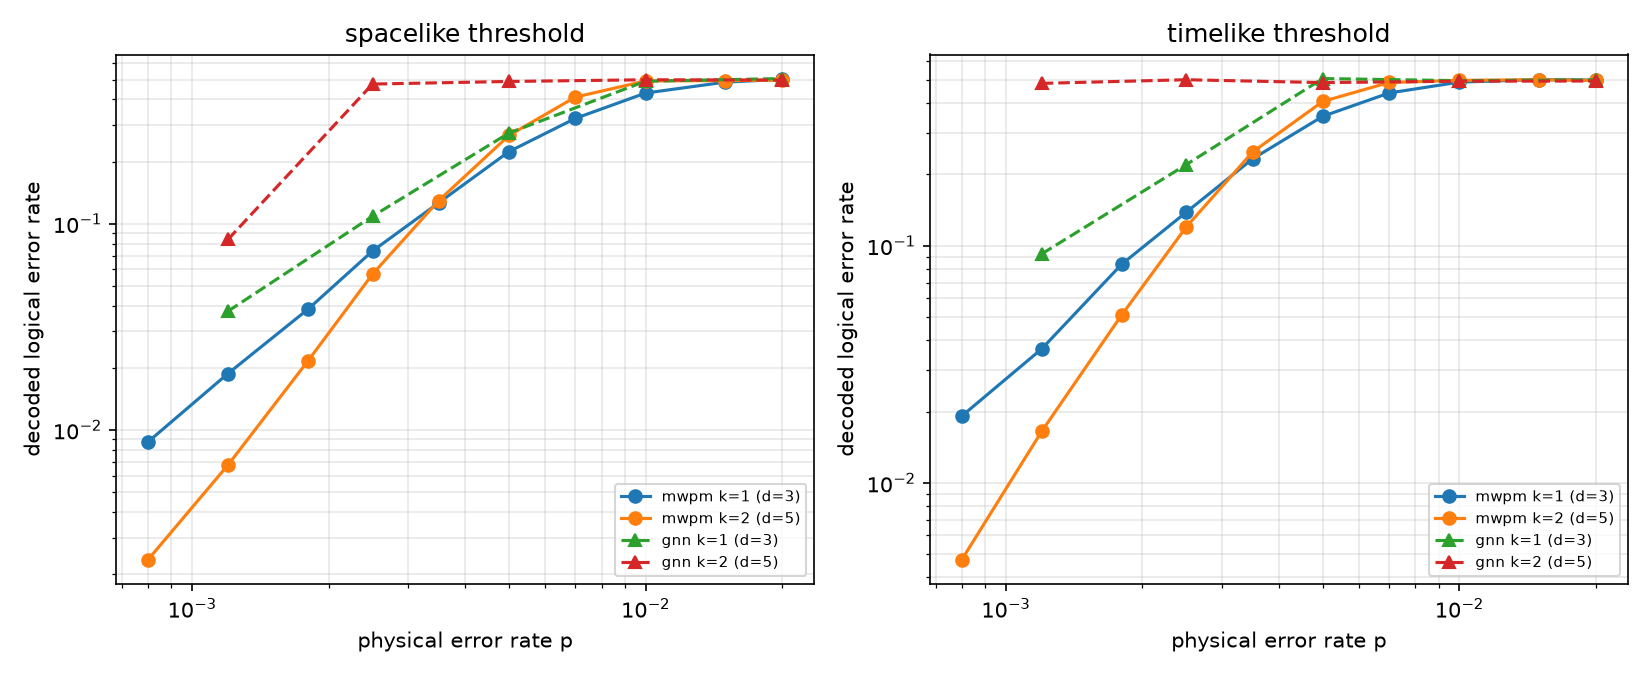
\includegraphics[width=0.95\textwidth]{timelike_threshold.png}
\caption{Spacelike (left) and timelike (right) logical error rate vs.\
physical error rate $p$, MWPM (solid) and GNN (dashed), $k=1$ and $k=2$.
MWPM shows the expected sub-threshold crossing; the GNN does not, in this
swept range.}
\label{fig:threshold}
\end{figure}

\subsection{Latency (E8)}

At $k=1$, GNN inference (GPU) is roughly $5\times$ faster per batch than
MWPM (CPU); the gap narrows sharply at $k=2$ as the larger merged-patch
graph increases per-batch GNN cost more than it increases MWPM's matching
cost (\texttt{results/main\_table.md}). We report both CPU and GPU numbers
where available; see that file for the full sweep. This was measured with a
capped, fixed batch size independent of the shot counts used elsewhere in
this pass, since a single-batch ``latency'' number at tens of thousands of
graphs is not a meaningful measurement.

\subsection{Ablations (E9)}
\label{sec:ablations}

\begin{table}[h]
\centering
\small
\begin{tabular}{lrrr}
\toprule
Variant & Mean rate & Std & $\Delta$ vs.\ baseline \\
\midrule
Baseline (all components on) & 0.0622 & 0.0021 & -- \\
Region/phase features removed & 0.0620 & 0.0035 & $-0.0002$ \\
DEM edges removed (radius-only) & 0.0640 & 0.0021 & $+0.0019$ \\
Radius edges removed (DEM-only) & 0.0563 & 0.0016 & $\mathbf{-0.0059}$ \\
Shallower (4 layers vs.\ 6) & 0.0633 & 0.0021 & $+0.0012$ \\
Normalization removed & 0.0645 & 0.0042 & $+0.0024$ \\
\bottomrule
\end{tabular}
\caption{Leave-one-out ablation, $n=8$ seeds, 30{,}000 shots, 20 epochs.
Baseline matches E5's $0.0622$ exactly -- the same configuration through
two different code paths.}
\label{tab:ablations}
\end{table}

Two effects stand out from noise at $n=8$ (an earlier $n=3$ pass could not
resolve either): removing radius-based edges and keeping only
DEM-derived edges is \emph{better} than the combination
($-0.0059$, roughly $3\times$ its own std) -- radius edges may add
connections the DEM structure does not need -- and removing the
region/phase one-hot features is essentially a no-op ($-0.0002$), even
though those are, in principle, the features carrying lattice-surgery
structure. The model appears to lean on DEM/geometric edge structure more
than on the explicit region/phase labels at this scale. Normalization
removed ($+0.0024$) and shallower ($+0.0012$) are smaller, same-order-as-std
effects, directionally consistent with the hyperparameter search's own
preference for normalization and depth but not independently significant
here -- no hypothesis test is applied to any of these deltas
(\S\ref{sec:limitations}).

\section{Limitations}
\label{sec:limitations}

This section is a summary; \texttt{LIMITATIONS.md} in the repository is the
authoritative, more detailed version and is written to be trusted over any
claim here if the two ever disagree.

\begin{itemize}
\item The hand-rolled circuit builder does not work; every result here uses
  the TQEC backend.
\item Unequal-distance patches and independent routing width are
  unimplemented -- confirmed at the TQEC API level to require patching
  TQEC's own internals, not simply unattempted.
\item Region/phase labels are inferred from which ancillas are active only
  during a short interior span of rounds, not read from explicit TQEC
  metadata; verified at two code distances, not proven in general.
\item The GNN does not beat MWPM anywhere in this study, including after a
  real hyperparameter search, and does not show MWPM's distance-scaling
  behavior in the H4 threshold sweep.
\item $n=8$ seeds is a real improvement over an earlier $n=3$ pass but is
  still not large enough for a formal confidence interval; no significance
  testing or multiple-comparison correction is applied anywhere.
\item No comparison to any published neural decoder (e.g.\ AlphaQubit) or
  external baseline beyond MWPM and this repository's own union-find
  implementation; no real device noise model.
\item The E3 zero-shot regression was isolated to training scale rather
  than architecture (\S\ref{sec:results}) by a single controlled
  comparison (old architecture, new scale); this rules out one specific
  alternative hypothesis but does not by itself establish the causal
  mechanism (e.g.\ via representation probing or an explicit
  train/zero-shot correlation study across many scale settings).
\item No public experiment-tracking dashboard (W\&B is integrated but was
  never run against a live account).
\end{itemize}

\section{Conclusion}

Architecture determines whether a learned decoder can be evaluated on
lattice surgery at all: fixed-input MLP/CNN decoders cannot, a GNN can. That
structural result holds regardless of tuning. Accuracy is a harder story --
the GNN trails MWPM everywhere we measured it, including on plain memory
after a real hyperparameter search, and shows no distance-scaling advantage
in a direct threshold comparison. Surgery-specific training closes most of
the zero-shot gap, but more memory-only training -- independent of the
tuned architecture, isolated by a direct controlled comparison -- made
zero-shot transfer worse, a finding this paper reports rather than smooths
over, and one that complicates the very premise of treating E2 as a gate
worth optimizing. We see this as a foundation -- a working,
GPU-accelerated, reproducible pipeline with an honestly documented gap to
close -- rather than a finished result, and \texttt{LIMITATIONS.md} in the
accompanying repository is maintained as the living, authoritative account
of exactly what is and is not demonstrated.

\begin{thebibliography}{9}
\bibitem{alphaqubit} Bausch et al. \emph{AlphaQubit: Learned Decoder for
  Quantum Error Correction}. Nature, 2024.
\bibitem{horsman2012} Horsman, Fowler, Devitt, Van Meter. \emph{Surface code
  quantum computing by lattice surgery}. New J. Phys., 2012.
\bibitem{mld2026} \emph{Maximum Likelihood Decoding of QEC Codes}, \S4.3
  ``Decoding beyond memory experiments.'' arXiv:2605.17230.
\bibitem{realtime2023} \emph{Real-Time Decoding for Fault-Tolerant Quantum
  Computing}, \S E. arXiv:2303.00054.
\bibitem{mlsurvey2026} \emph{ML Approaches to Decoding Topological Quantum
  Codes}, \S4. arXiv:2608.15760.
\bibitem{latte2025} \emph{LATTE: spatially parallel lattice-surgery
  decoding}. arXiv, 2025.
\bibitem{parallel2024} \emph{Spatially parallel decoding for multi-qubit
  lattice surgery}. arXiv:2403.01353.
\bibitem{netdecode2024} \emph{Network-Integrated Decoding System for
  Real-Time QEC with Lattice Surgery}. arXiv:2504.11805.
\bibitem{tqec} TQEC. \url{https://github.com/tqec/tqec}.
\end{thebibliography}

\end{document}
